% - Report for the CS 296 Project by Group 14
% - Report contains analysis of profiler output and also a comparison between the targeted Rube Goldberg machine and the one we've built.

\documentclass[11pt] {article}
\usepackage[top=1in, bottom=1in, left=0.5in, right=0.5in]{geometry}
\usepackage{times}
\usepackage{graphicx}
\usepackage{enumitem}
\usepackage{subfigure}
\usepackage{amsmath}
\usepackage{float}
\usepackage{cite}
\usepackage{graphicx}
\setitemize{noitemsep,topsep=0pt,parsep=0pt,partopsep=0pt}
\makeatletter
\setlength{\@fptop}{0pt}
\makeatother
\bibliographystyle{plain}
\begin{document}
\title {Analysis of Profiler Output and the Rube Goldberg Machine}
\author 	{	Vivek Agarwal \\
				110050042 vivekcse@cs.iitb.ac.in \\
				\and
				Manoj Tadepallilakshmi Datta \\
			 	110050063 manojtld@cse.iitb.ac.in \\
			 	\and
			 	C. Yeshwanth \\
			 	110050083 yeshwanth@cse.iitb.ac.in}
\date{\today}
\maketitle

\section {Introduction}

In this report, we analyze the profiler output obtained in the same way as was obtained in Lab 9 except that the 
Rube Goldberg machine code was used instead of the dominos code that was used in the previous profiling exercise.
We also compare our target Rube Goldberg machine to the one we've built and present reasons for the deviation.

\section{Plot Analysis}

\subsection{Plot 1} \cite{1,2}

\begin {figure} [ht]
\begin {center}
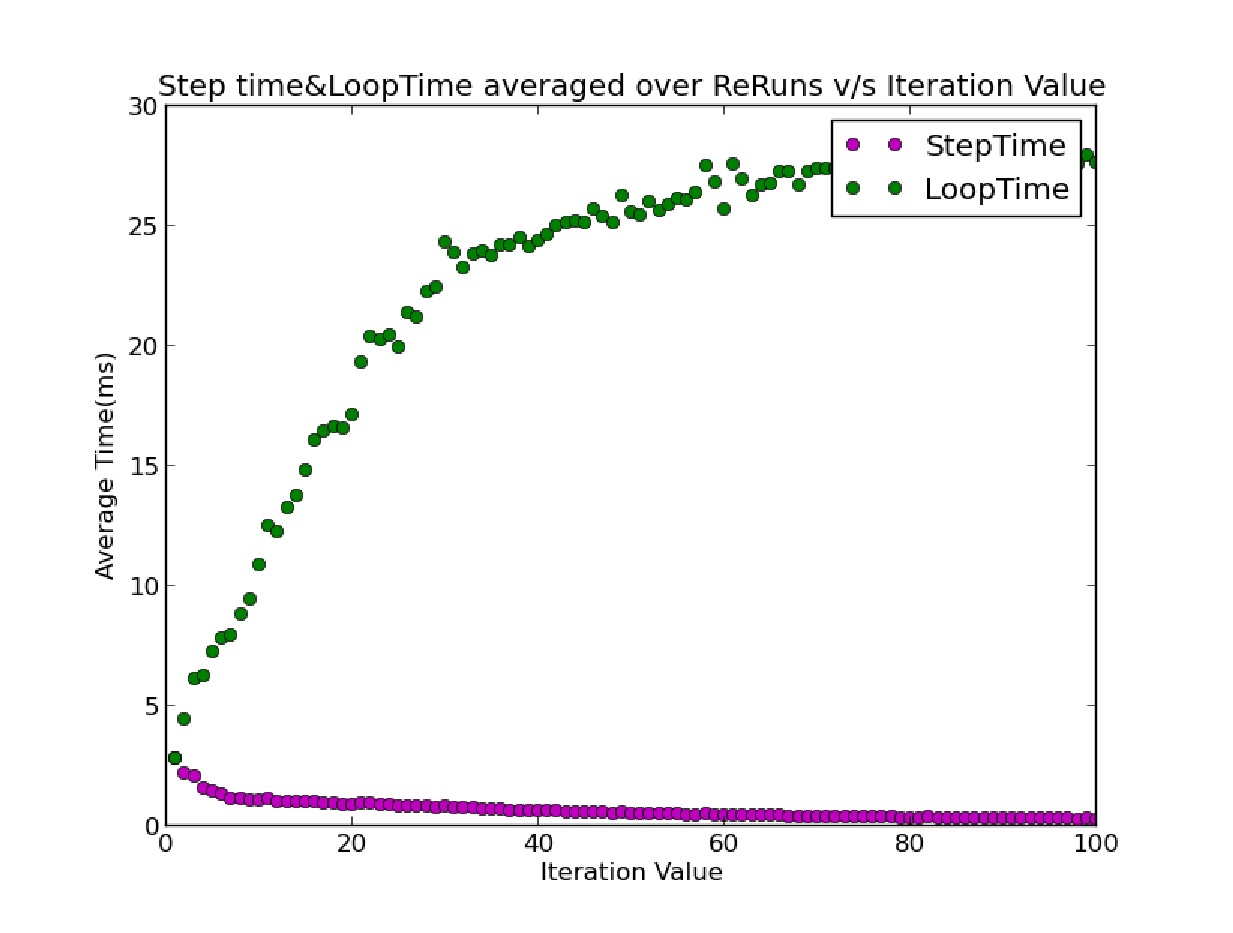
\includegraphics[scale = 0.35] {1.eps}
\end {center}
\caption {Plot - 1}
\end {figure}


In the plot for lab 9, we observed that the average Step time decreases while the total loop time
increases with the number of iterations. The graph obtained in the case of the Rube Goldberg machine
was very similar with a change in slope being observed in the total loop time as was the case with
the dominos code. Again, we attribute both to the fact that linux prioritizes programs. Again 
programs with higher priorities seem to be given more resources and we believe that this is the 
cause of the speed up. The more resources for roughly the same computation per iteration cause 
the program to run faster and this results in the change in slope and the decreasing average Step\cite{2}
time per iteration.

\subsection{Plot 2}\cite{1,2}

\begin {figure} [H]
\begin {center}
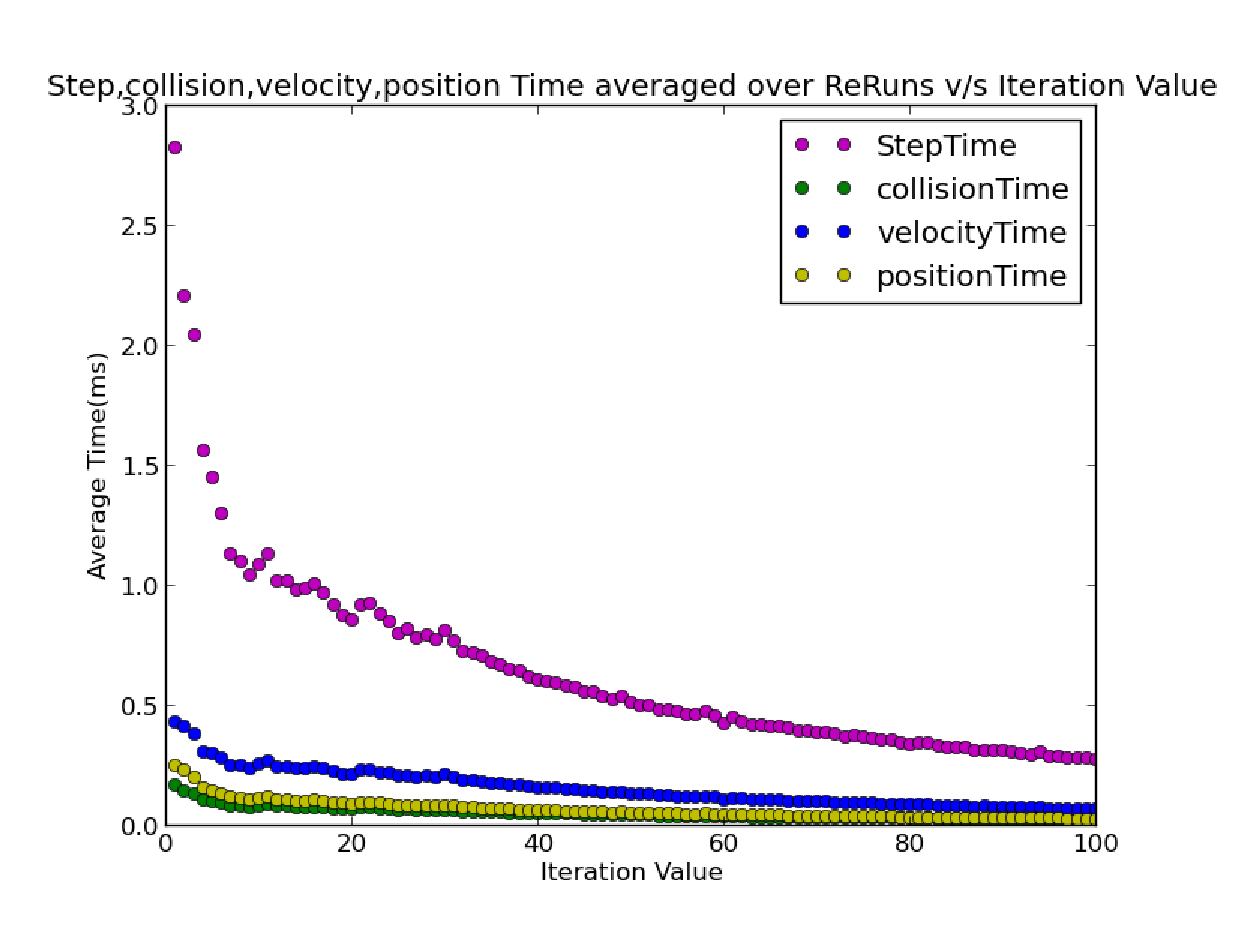
\includegraphics[scale = 0.35] {2.eps}
\end {center}
\caption {Plot - 2}
\end {figure}

Again, the results of the profiling data for the Rube Goldberg machine are very similar to the results 
of Lab 9. The reason for this behavior is again attributed to the same causes that were mentioned in the
previous section that Linux prioritizes it's programs and allocates more resources to the ones with
higher priority. 

\subsection{Plots 3a and 3b}

\begin {figure} [ht]
\begin {center}
\subfigure[Plot 3a]{\label{fig:edge-a}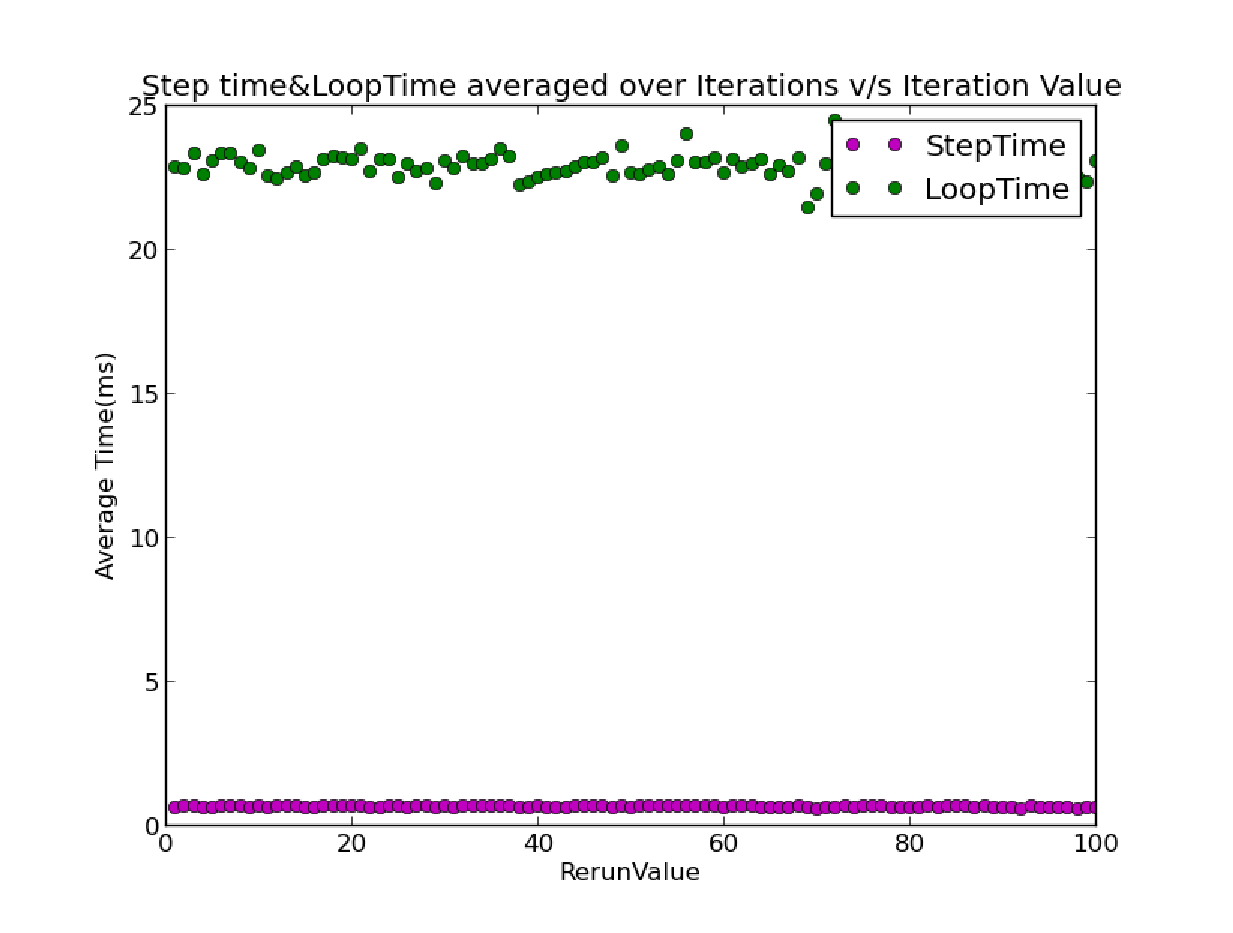
\includegraphics[scale=0.35]{3.eps}}
\subfigure[Plot 3b]{\label{fig:edge-b}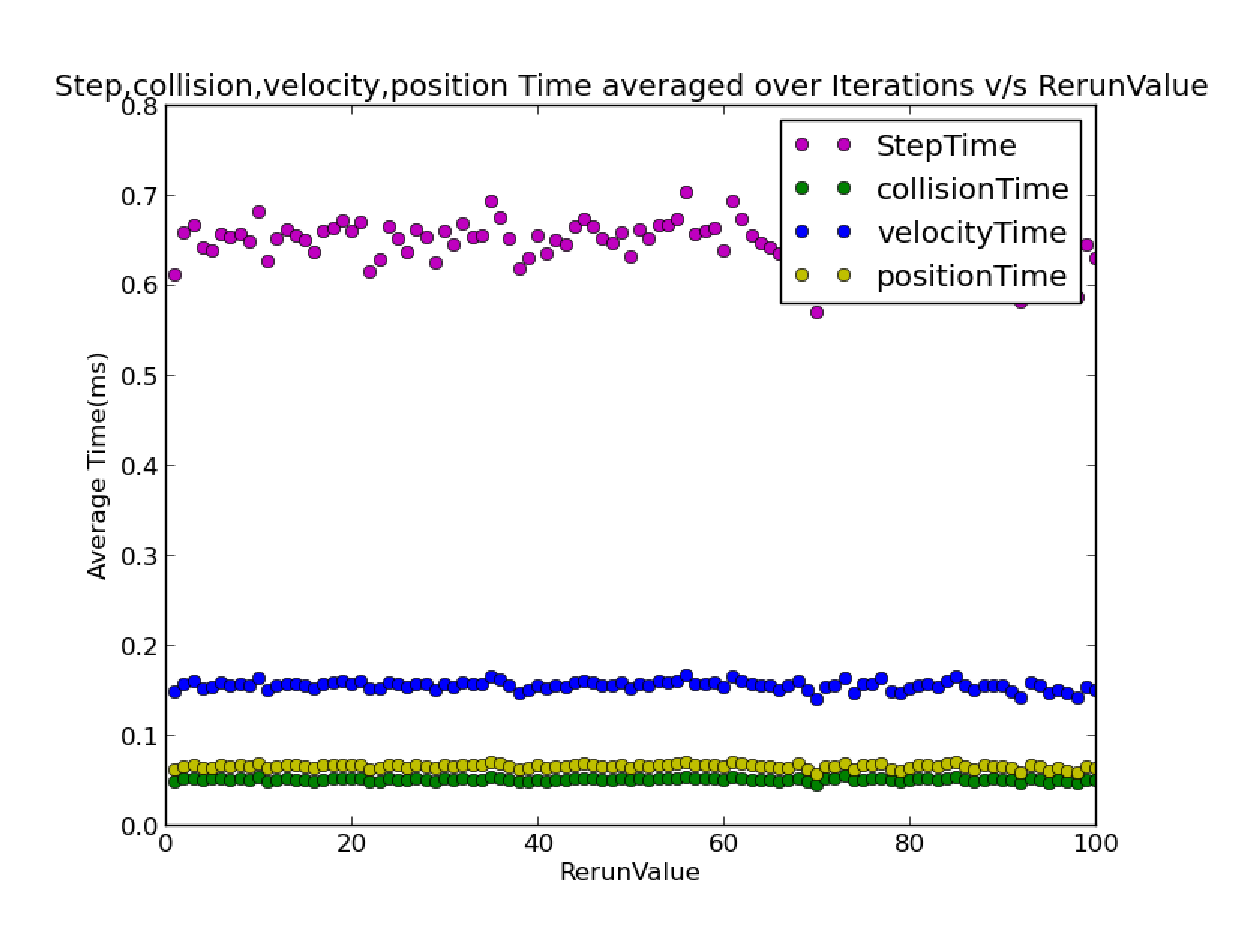
\includegraphics[scale=0.35]{4.eps}}
\end {center}
\caption {Plots 3a and 3b}
\end {figure}

The results of this plot yield little information about the functioning of the linux kernel.
The plots are basically straight lines which shows that re-run values seem to have little to
no effect on the performance of the program. This could maybe show that linux does not 
maintain information about the previous time that a program was run and the type of computations
that the program carried out.\cite{rube}

\subsection{Plot 4}

\begin {figure} [ht]
\begin {center}
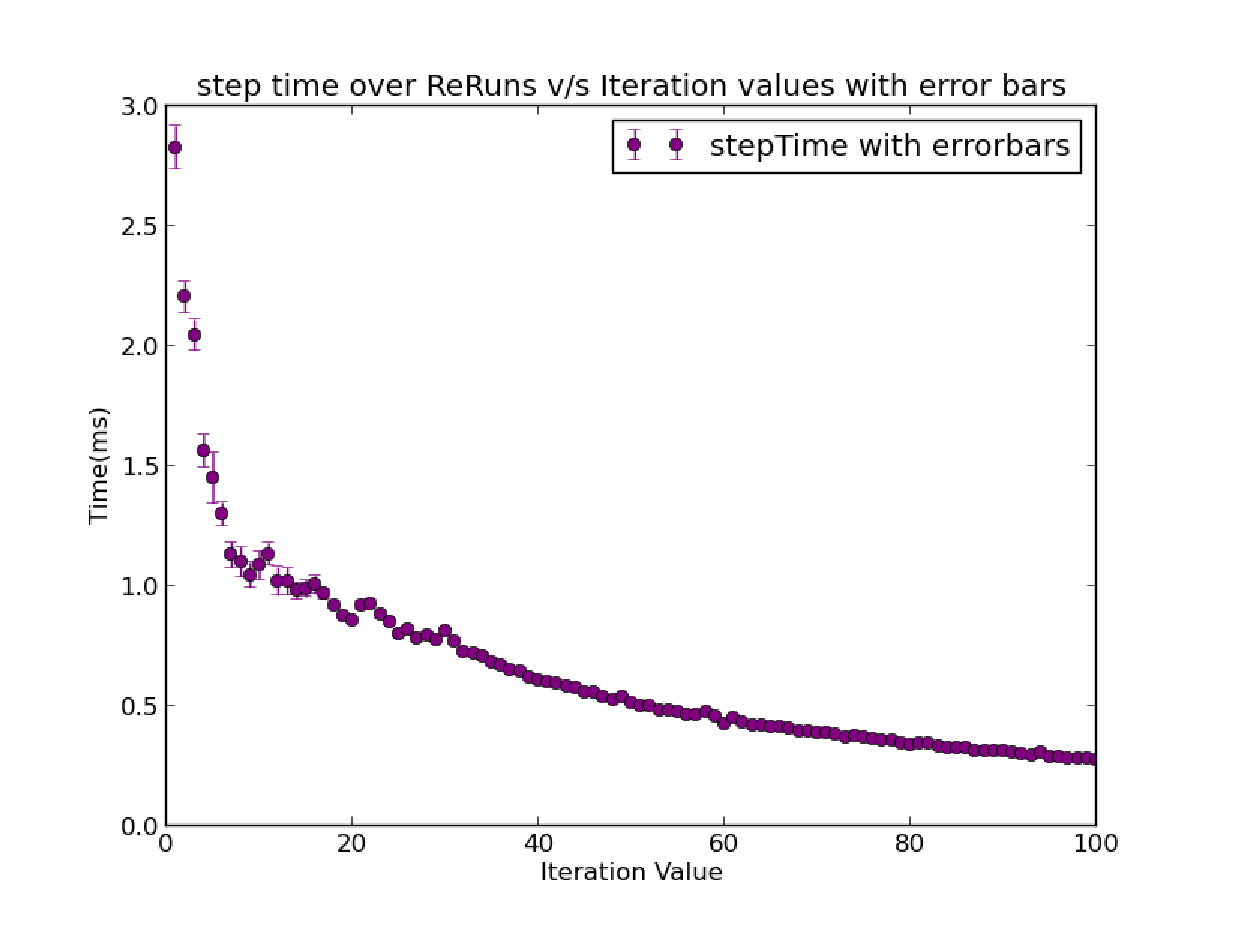
\includegraphics[scale = 0.35] {5.eps}
\end {center}
\caption {Plot - 4}
\end {figure}

This particular graph yields very interesting results as it shows that it is not only the average 
step time that drops with iteration values but also the variance in the average loop time. The 
decrease in average step time has been explained in the preceeding sections. We believe the 
variance decreases with the number of iteration values because of firstly, the fact that the 
variance of the mean decreases with the number of samples that were taken and secondly as the
number of iteration values increases, the resources allocated to the program running the same
iteration over different reruns tend to stabilize and this reduces the variance in the average
step time. This is similar to the results of Lab 9 and while they in no way prove the statements
that we have just made, it at least proves that the observations are general and not something
specific to the dominos code.

\subsection{Plot 5}

\begin {figure} [ht]
\begin {center}
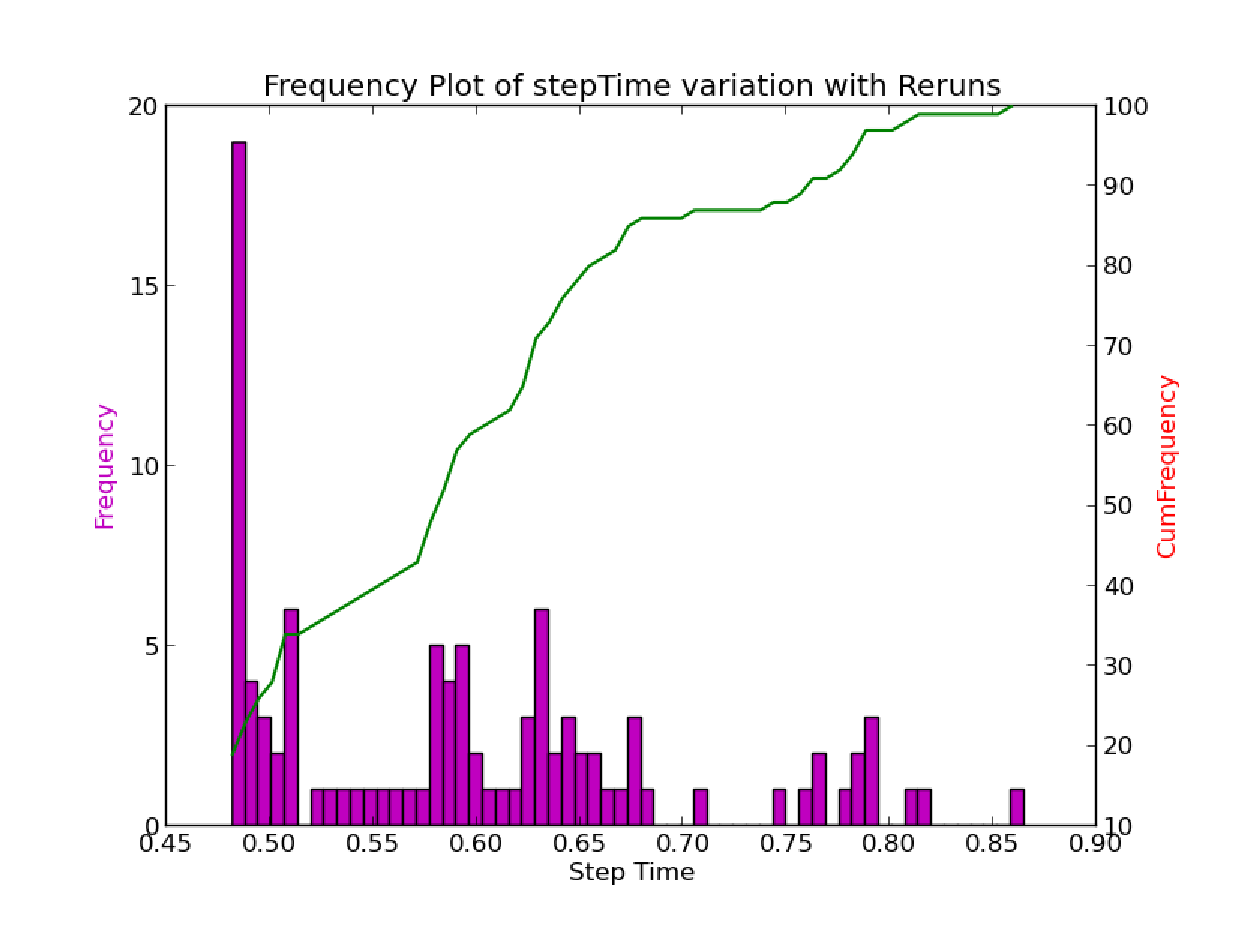
\includegraphics[scale = 0.35] {6.eps}
\end {center}
\caption {Plot - 5}
\end {figure}

In this graph, the distribution of average step times for an iteration number of 42 is a lot more 
random than the one we had obtained for Lab 9. A particularly high peak is noticed near the lowest
range of average step times but nothing substantial enough for us to draw reasonable conclusions.

\section{Performance Gains Upon Using the -O3 Flag}\cite{3,4}

Based on the results of Lab 9, we ran the simulation for 50000 iterations and we found that this
was sufficient to differentiate the optimized version of the code from the non-optimized or the
debug version. The results of the profiler for 50000 iterations yielded a speed up of about 5 times
and significant differences were observed in the call graphs. Since the behaviour of the graph is
not much different between the two cases (dominos and the Rube Goldberg Machine), we present
similar arguments for the case of the Rube Goldberg Machine as well. As we saw from the data
the function solve velocity constraints which took up 0.68 seconds to run and formed 6.92 \% for 
the dubug-versiion of the code in one run took 0.25 seconds to run in the optimized version and 
comprised 12.5 \% of the total running time.

\subsection{Difference in the Analysis Files}

In both versions the functions taking the largest amount of time was the SolveVelocityConstraints() in
b2ContactSolver.cpp and in the joint computation. The distinction between the two runs with iteration values at and above 5000 was
the absence of several functions relating to the Vector class b2Vec2. One of the optimizations of 
the -O3 tag is the one that includes smaller functions as inline functions. This increses the size of
the executable but greatly speeds up the execution of the program as the program pointer does not need
to be redirected each time a function is called. There are several pointer references to the points 
variable in the function belonging an object called vc which is accessed repeatedly and the
optimized version does not duplicate the work performed in this process. There are also several cases
within the function where objects are created within the loop body but are destroyed subsequently.
Memory is allocated for these objects during an iteration and is deallocated after the current 
iteration. This can be avoided by putting the objects outside of the loop as memory would not need
to be allocated repeatedly within the loop. There is also the case where a memory address is accessed
repeatedly within a loop and this causes repeated computation that can be avoided.

\subsection{Differences in the Call Graphs}

\begin {figure} [ht]
\begin {center}
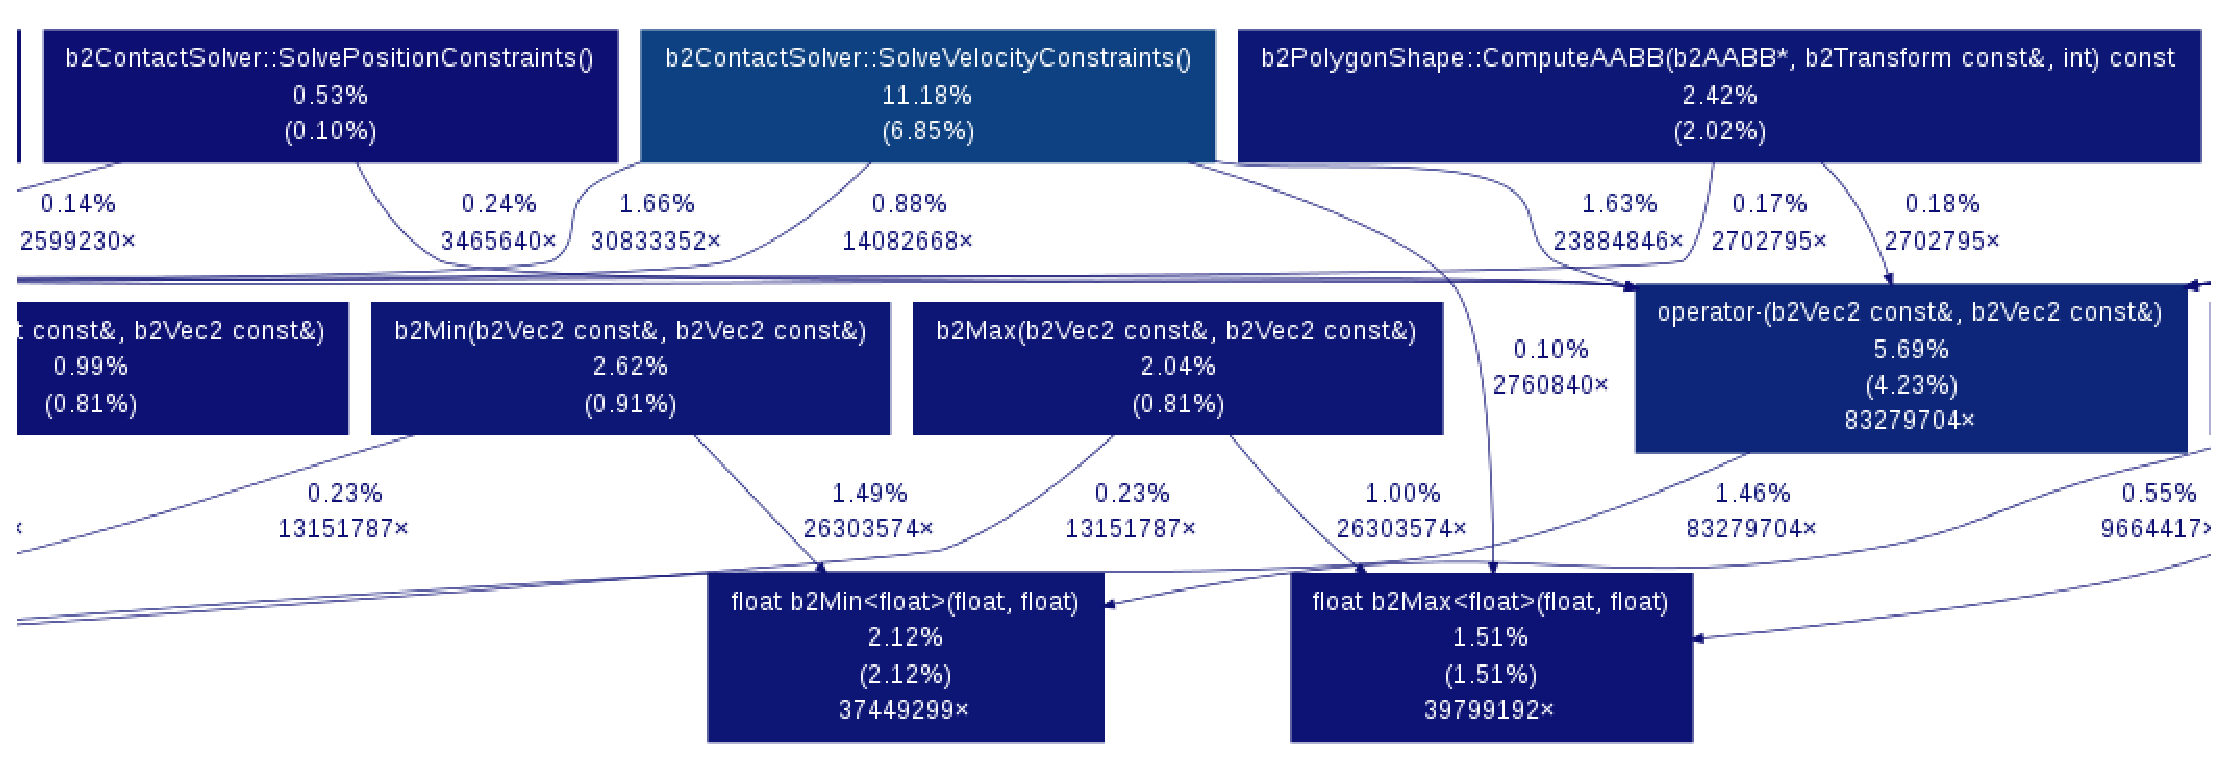
\includegraphics[scale = 0.4] {debugProfile.eps}
\end {center}
\caption {Non-Optimized}
\end {figure}

\begin {figure} [ht]
\begin {center}
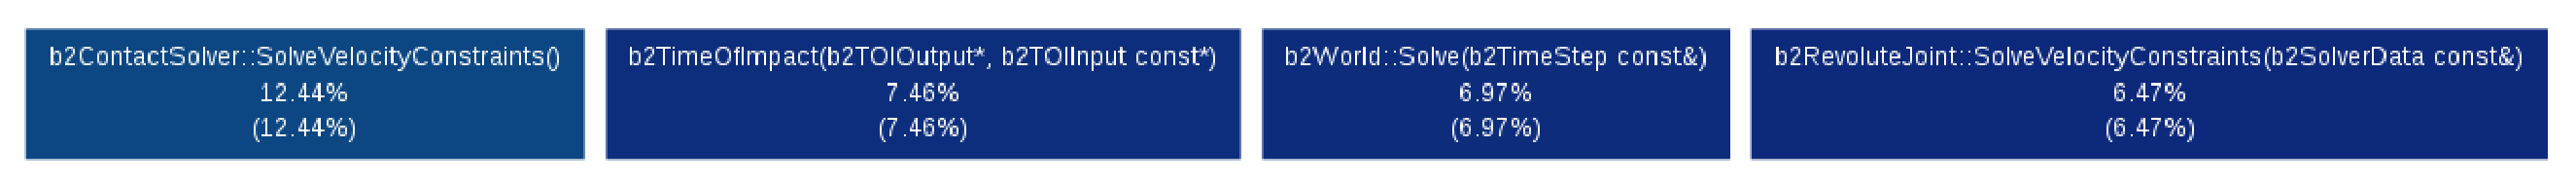
\includegraphics[scale = 0.4] {releaseProfile.eps}
\end {center}
\caption {Optimized}
\end {figure}

A single block of the call graph shows the fraction of the time that the function was running as
a fraction of the total running time of the program. Outgoing edges represent the calls made by the
function within the block to other functions that were called during the running of the function. The 
two values that are included with the block of a function are the amount of time the function was on the
program stack and the amount of time it was on top of the program stack. The call graphs also convey the same information
 as the analysis files. The show that a large number of functions relating to b2Vec2 have been made 
 inline at the cost of space but improve the running times of the program. The Call Graphs do not
 show much distinction between the two versions for small iteration values similar to the Analysis 
files but on much larger iteration values above 5000, a difference was observed in the distribution 
of time for various times. It showed that some of the functions mentioned above (operator+, operator*, 
dot products, cross products, etc) were called in the order of $10^{6}$ times and the time spent in 
referncing these functions was a significant contributor to the discrepency between the two versions. 
Both the Call Graphs again showed SolveVelocityConstraints() to be the most expensive function and 
this was the function that we investigated primarily to suggest improvements to the existing code. 

\section{Optimizations}

Several optimizations can be made to the code to improve it's running time. We found instances within
the function SolveVelocityConstraints() where clever optimizations could drastically speed up run times.
Some of the optimizations that we found are listed below:

\subsection {Inline functions for b2Vec2 classes}

As noticed in both the call graphs and the analysis files, we saw that an enormous amount of time was 
wasted when the functions weren't made inline as these functions were called on the order of $10^6$
times. This situation can be greatly improved my making certain functions corresponding to the b2Vec2
class like the constructor, dot product, the operator* and the cross products inline as these would 
reduce the need to redirect the program pointer to the code that corresponds to these functions and
reduce the load on the program stack. This simple optimization is responsible for a large amont of
the savings that are obtained with the -O3 flag.

\subsection {Reducing Object Member Access Within Loops}

The points member of vc is accessed repeatedly within the for loop corresponding to SolveVelocityConstraints().
This situation can be made better when the value is stored before the loop and is incremented with a ++ 
increment operator within the for loop as this is a cheaper operation that incrementing the value of the 
pointer with a "+ (int)variable" operation. The for loop can be re-written to remove the repeated access
of the points variable and to reduce the number of "+ j" operations performed on it. This occurs in
 several other cases in the code following the one mentioned in SolveVelocityConstraints(). This can be
 changed to the more conservative version mentioned here.
 
\subsection {Memory Allocation within Loops}

Memory is allotted for a lot of variables within the loop and this memory is allocated dynamically (ex. 
indexA and indexB). This memory is re-allocated in each iteration of the for loop. This memory is 
allocaed and de-allocated in each iteration. This work can be reduced by allocating space for the 
variables before the loops as this reduces the need to re-allocate memory during the iteration and
these variables are accessible inside the for loop for any manipulation that might be needed. The
downside to this process is that this memory will not be de-allocated as long as this particular 
function call is within the program stack and this could cause problems for memory intensive
processes later in the function.

\subsection {Mathematical Simplifications}

There are also instances within the program where the amount of calls to comparatively heavy multiplication
and cross product computations can be reduced by utilizing basic mathematical properties of the operations
mentioned before. The distributive properties of multiplication over addition and the formula for computing
triple cross can simplify the computation of certain values within the SolveVelocityConstraints() function.
Specifically, the vA, wA, vB and wB can be simplified by using the distributive properties of integer
multiplication and scalar cross product. The computation of dv1 and dv2 in the later segments of the code
involve a triple scalar product upon substitution of the value of wB and similar variables in the code and
this can be simplified further leading to a more efficient implementation. In the first case the value of
P can be accumulated through the loop and the cross product can be calculated once after the loop as cross
products are expensive computations and additions are relatively faster (O($n$) for addition vs O($n^{1.59}$)
for multiplication).

\begin {equation} 
a\times(b+c) = a\times b + a \times c
\end {equation}

\begin {equation} 
a\times(b\times c) = (a.c)b - (a.b)c
\end {equation}

\subsection {Profiling Conclusions}

From the profiling data for the Rube Goldberg machine, we noticed that most of the optimizations that we had observed
in the code right from making functions inline to adjusting memory allocation within loops was already being handled by
the -O3 optimization flag. There doesn't seem to be any significant gain in performance that we could achieve by 
investigating the code further. Therefore, we feel that at our current level of knowledge, it is difficult to further
improve on the optimizations made by the -O3 flag and have thus, left the code unchanged. All of the changes observed
in the solvevelocityconstraints functions can also be made in the other functions Solve and TimeOfImpact functions to 
improve performance as seen in the call graphs which indicate similar branching in the function calls.

\newpage

\section {The Rube Goldberg Machine}\cite{rube,5}

\subsection {The Goal of The Rube Goldberg Machine}

Our Rube Goldberg machine attempts to erect a tent through a convoluted process which starts with a simple dropping
of a ball from a height which sets into motion a series of pulleys, pendulums and levers to eventually erect a tent
that is placed on the ground at the bottom of the simulation. 

\subsection {What Makes the Machine Interesting}

One theme common to almost all the Rube Goldberg machines that we encountered online was sequentiality. In every 
machine, we found that there was at most one section of the machine that was actively involved inmoving closer 
to the end goal of the machine. We wanted to make a Rube Goldberg machine that was not sequential which 
essentially meant having to parallel branches to the machine that would come together at the end to erect the
tent. To make the machine symmetric was an obvious way to achieve this goal and this also ensured synchronicity 
between the two processes without any extra effort. This was also easy to reconcile with the goal of the machine
as the tent was symmetric in nature. Also, we have a bull. And he's angry.

\subsection {The Design of the Rube Goldberg Machine}

The machine starts with the dropping of a single ball from the roof of the simulation, persumably by some tired and
weary camper in need of rest. This sets in motion two balls that it collides with in opposite directions which roll 
across the shelf at the top of the simulation and collide with a revolving bar hinged to the edge of the shelf. 
This bar rotates about this hinge and hits another (no prizes for guessing) ball. To stop the two stray balls from
the top of the simulation from falling off the shelf and wrecking the poor camper's tent, we improvised on the
design of the shelf to introduce two vertical bars to stop the balls falling off (these would eventually form the
horns of the bull but more on that later). The two other balls now roll off the shelf to set in motion a series of
interlocking revolving bars and subsequently fall into another improvisation forming the nostrils of the bull giving
him his charming personality. Now back to the simulation, the ball set in motion by the revolving bars falls into
the frustum which pushes it onto a pulley. The bar at the other end of the pulley rises and sets yet another
revolving bar in motion. The ball of the aforementioned bar, falls onto a smooth slope which guides the ball into
the path of a pendulum which is powerless to do anything about it. The hapless pendulum then gets clobbered onto 
the set of dominos lined up which fall like . . . well . . . dominos. The last domino falls onto a ball which rolls
down a slope and falls on one of the arms of a See saw at the bottom of the simulation. The other end of the See-saw
holds a small square box which is launched into the air by the heavy ball. This square box is redirected by an 
aptly placed static bar into a small container connected to a pulley connected to the tent thus raising it for
our (now) happy traveller.

\subsection {Deviations from Original Design}

\begin {figure} [ht]
\begin {center}
\subfigure[Original]{\label{fig:edge-a}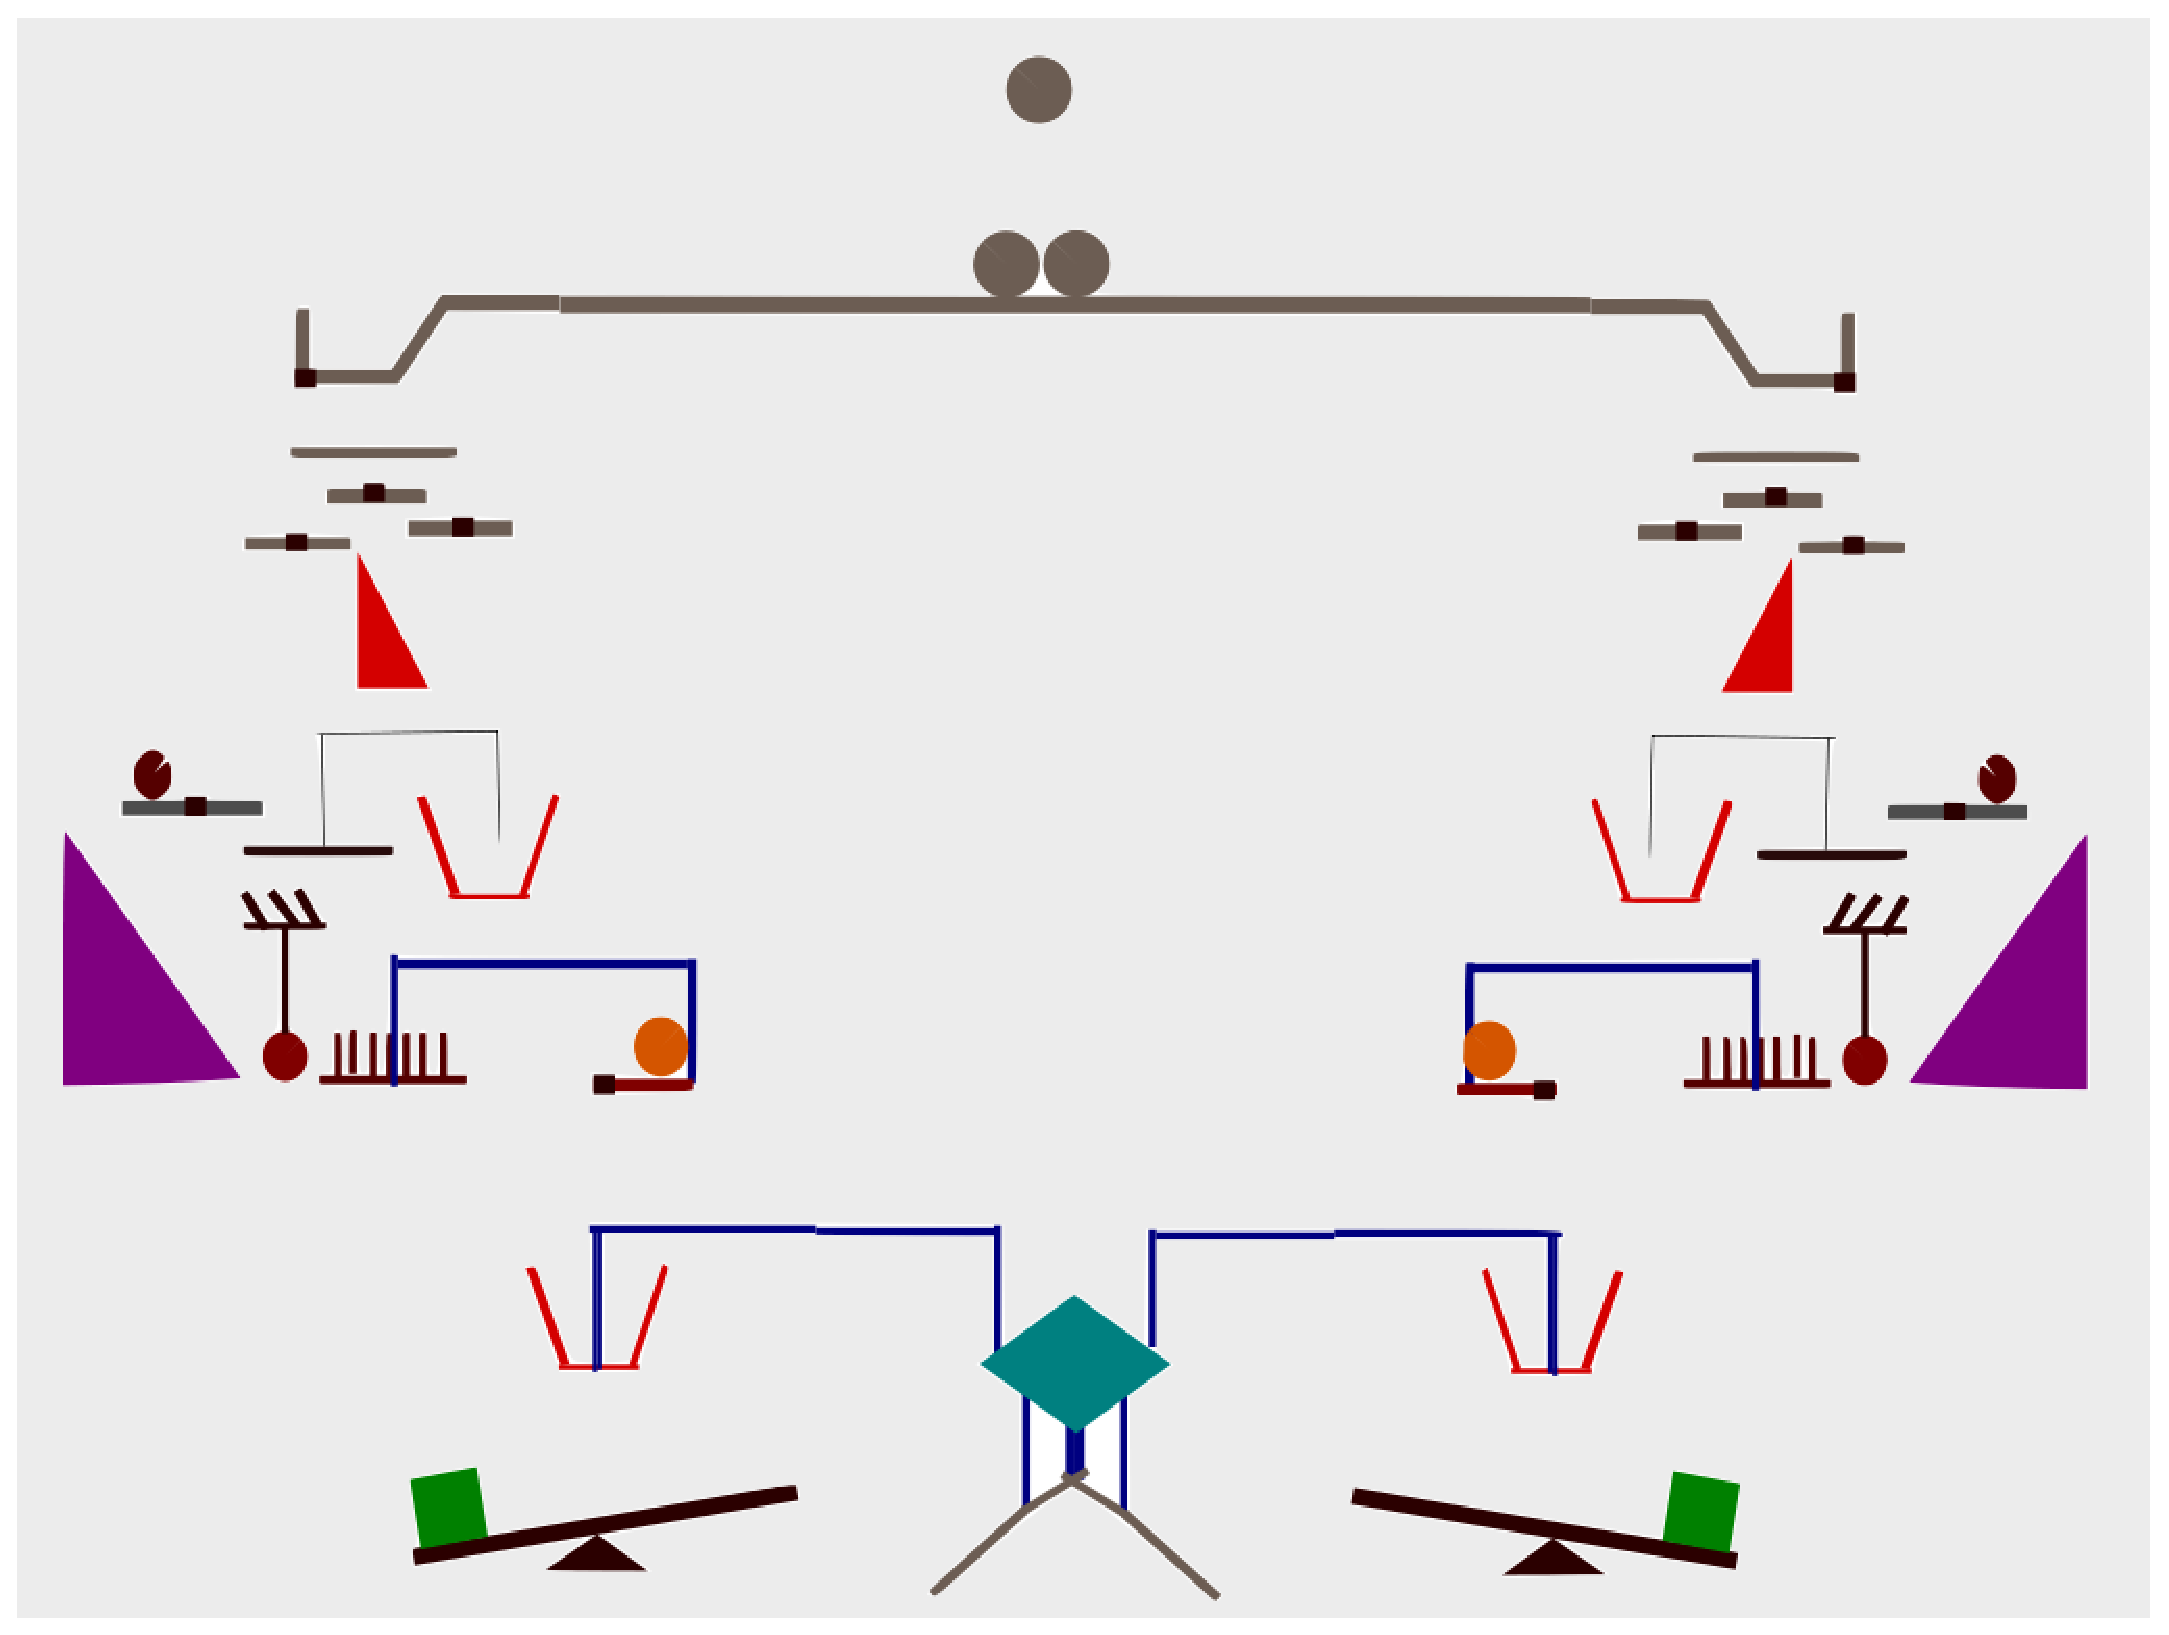
\includegraphics[scale=0.25]{original.eps}}
\subfigure[Implemented]{\label{fig:edge-b}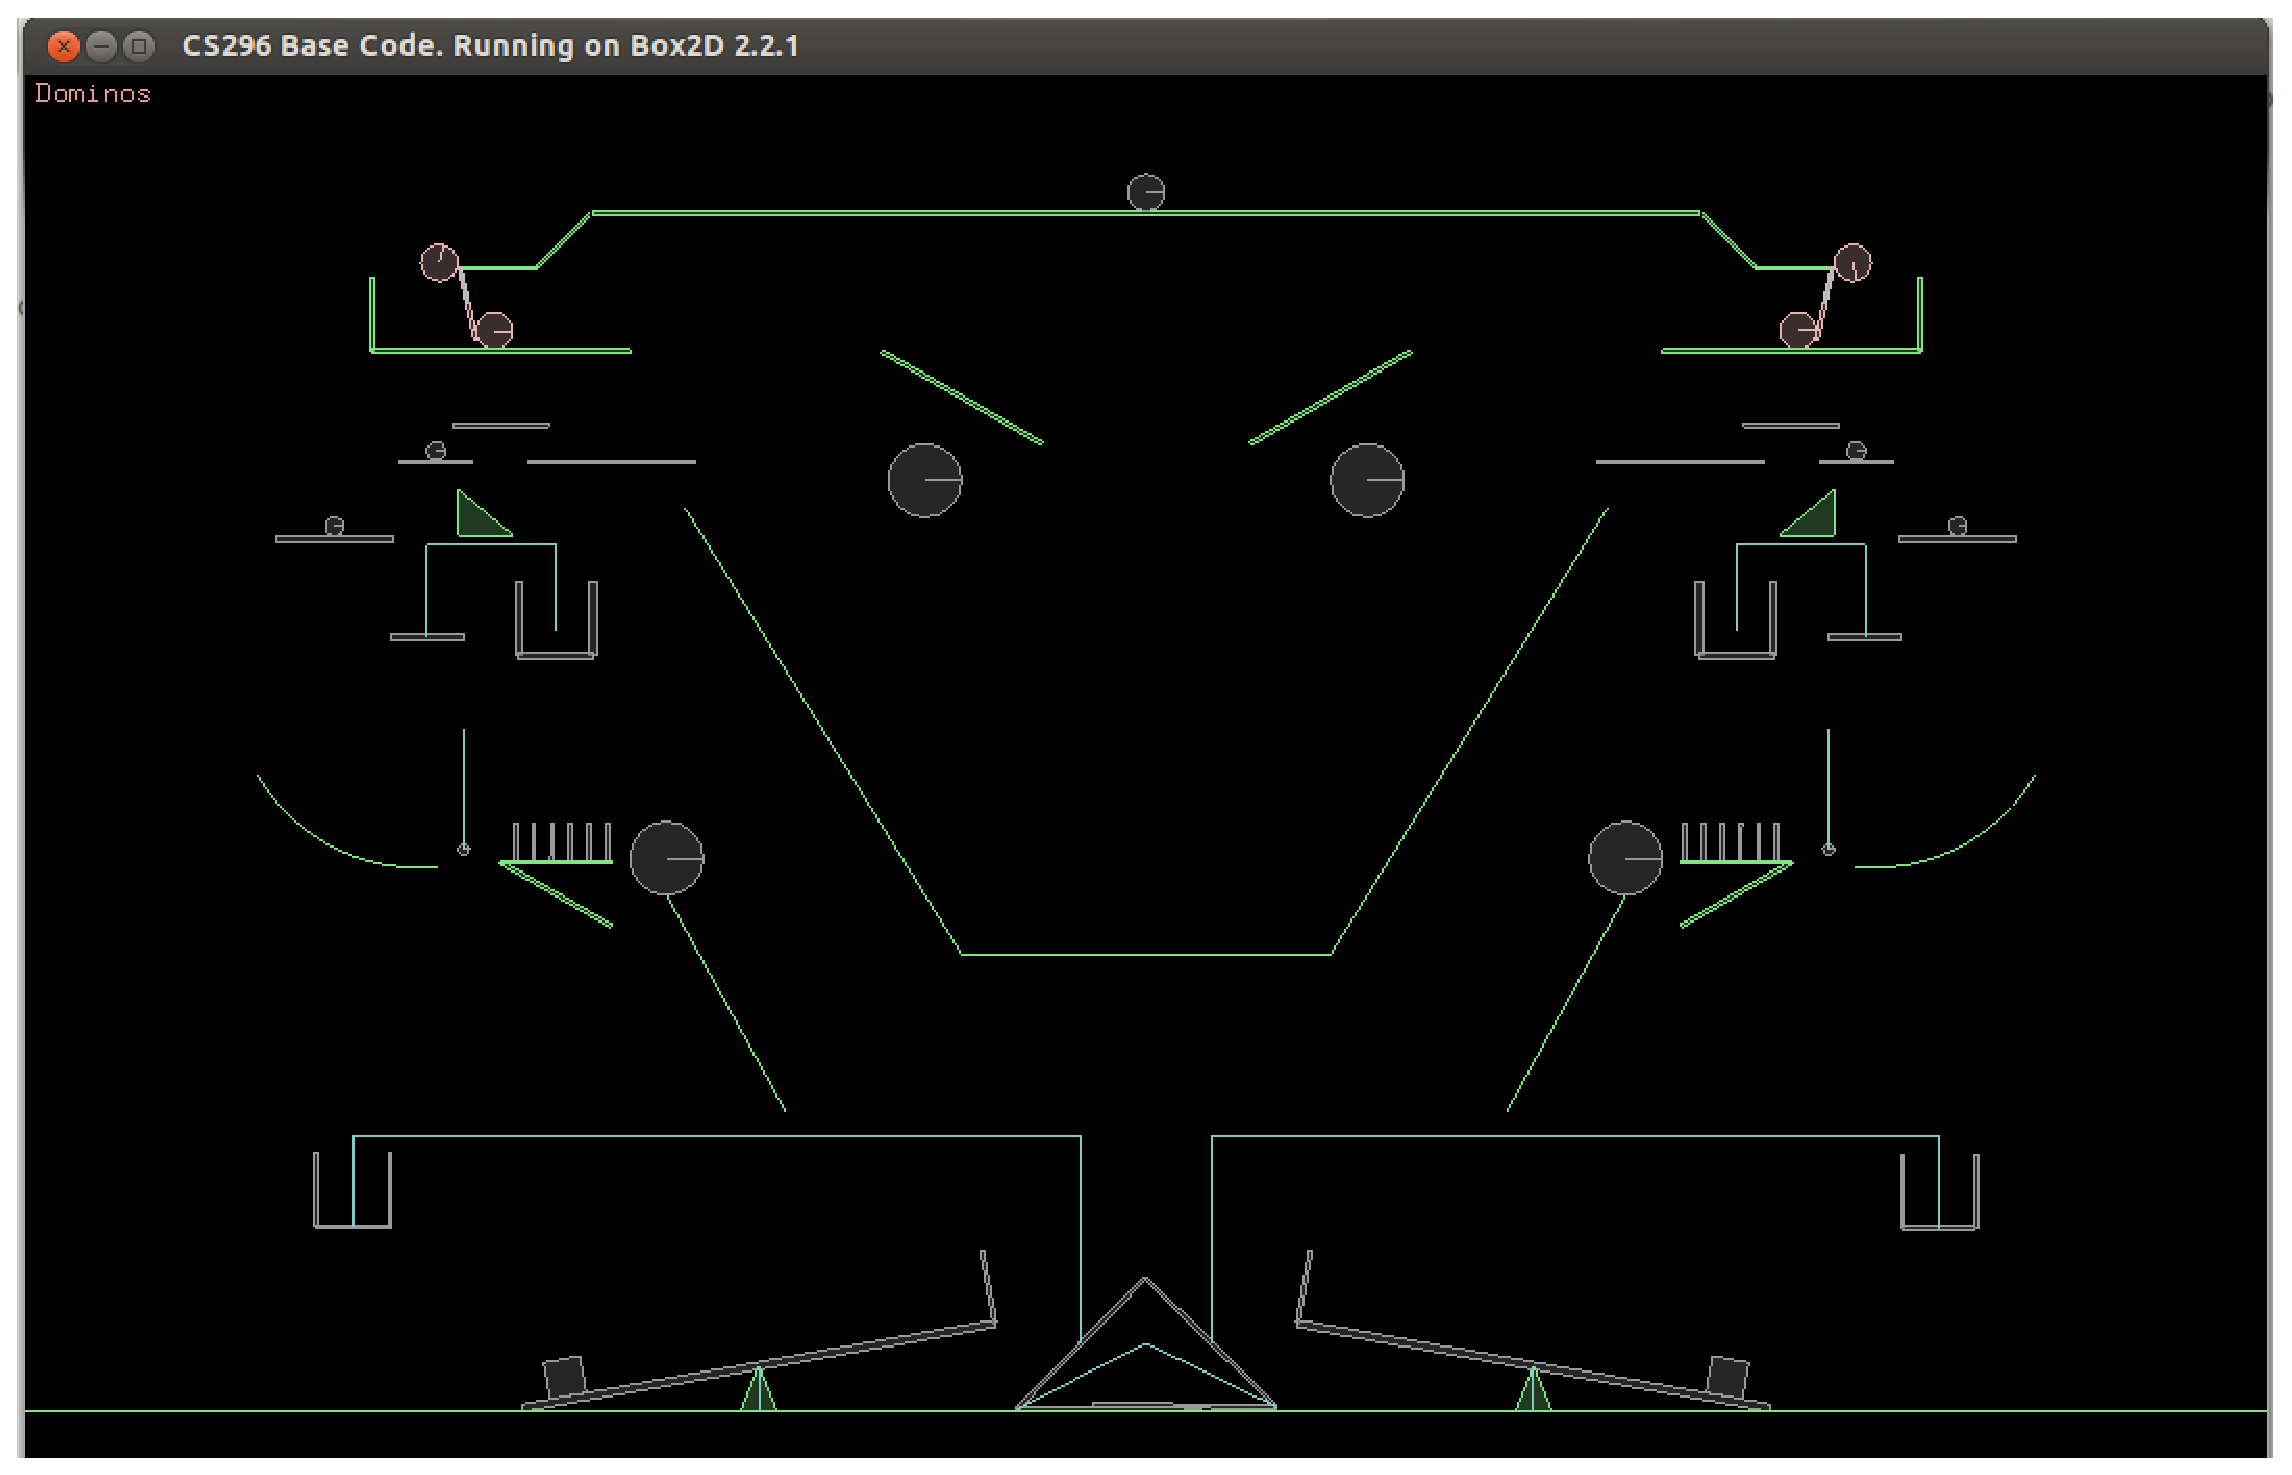
\includegraphics[scale=0.25]{implemented.eps}}
\end {center}
\caption {Original and Implemented Machines}
\end {figure}

In this section, we will contrast the Rube Goldberg machine that we've implemented from the one that is present on
the Group home page. We will begin by noting the similarities between the two. As you can see from the diagram, we
have not deviated significantly from the design that we started out to build. The machine still performs the 
same function using mostly the same tools that we used in the original. One immediately noticable difference is 
the face of the bull in the simulation. While this may seem completely at odds with the purpose of the machine, it
still serves as an amusing backdrop to the simulation. The reasons for the deviations that you do see in the
picture is to prevent stray parts in the Rube Goldberg machine from interfering in the simulation after they have
served their purpose. As you can see in the simulation, the bull stops the two balls that fall from the highest
 shelf in the simulation from falling on the ground and potentially leading to disaster for our tent. More appendages
 of the sort can be noticed in the See-Saw structures at the bottom of the simulation where we've taken care to 
 make sure that the heavy balls that land on the See-Saw do not roll off the See-Saw and collide with the light tent
 which could cause the tent to behave unpredicatably. We've also tried to not reuse the same pieces too much in the
 simulation as we felt that this would make it a boring experience for the viewer. With this in mind, we've replaced
 the large purple wedge in the original simulation with a curve which adds variety to the machine but is also
 much more aesthetically pleasing than the large, clunky wedge. One more difference between the two simulations 
 is in the way the box meant to counterbalance the tent falls into the container at the other end of the pulley.
 In the original simulation, we had hoped to achieve this by launching the box into the air and directly into the
 container from the See-Saw system at the bottom. But after much trial and error, we found that we could only
 launch the box vertically from the wedge we had constructed despite significant effort spent in manipulating
 the different parameters of the simulation. We accounted for this by placing a slab directly above the box tilted
 at an angle to redirect the box into the container at the end of the pulley. The parallelogram above the house was
 also eliminated as it did not serve any practical purpose and took up important vertical space in the simulation.
 The pulley mechanism for dropping the heavy ball onto the See-Saw was removed partly because it took up more space
 than we had in the simulation and also because it would've formed the third such pulley mechanism in the machine
 which would seem redundant from the perspective of a third party viewer. 
 
\subsection {Concluding Remarks on the Rube Goldberg Machine}

As you can see from the figures that we've included with this report, we have tried to mimic the original Rube
Goldberg machine as closely as possible while at the same time we have taken the liberty to change the
simulation subtly to make it aesthetically more pleasing and practically more viable. The inclusion of the
bull satisfies both those properties while the other modifications were simply to tie up the loose ends of 
the simulation together. All in all, we have constructed the Rube Goldberg machine that we set out to build
without significantly deviating from the original design and for the most part we have succeeded in our effort.
 
\bibliography{ref}
\end{document}
